%% $RCSfile: proj_proposal.tex,v $
%% $Revision: 1.2 $
%% $Date: 2010/04/23 02:40:16 $
%% $Author: kevin $

\documentclass[11pt, a4paper, twoside, openright]{report}

\usepackage{float} % lets you have non-floating floats

\usepackage{url} % for typesetting urls

%  We don't want figures to float so we define
%
\newfloat{fig}{thp}{lof}[chapter]
\floatname{fig}{Figure}

%% These are standard LaTeX definitions for the document
%%
\title{Web Application Key Management Progress Report}
\author{Sriram Venkatesh}

%% This file can be used for creating a wide range of reports
%%  across various Schools
%%
%% Set up some things, mostly for the front page, for your specific document
%
% Current options are:
% [ecs|msor]              Which school you are in.
%
% [bschonscomp|mcompsci]  Which degree you are doing
%                          You can also specify any other degree by name
%                          (see below)
% [font|image]            Use a font or an image for the VUW logo
%                          The font option will only work on ECS systems
%
\usepackage[image,ecs]{vuwproject} 

% You should specifiy your supervisor here with
%     \supervisor{Firstname Lastname}
% use \supervisors if there are more than one supervisor

% Unless you've used the bschonscomp or mcompsci
%  options above use
\otherdegree{Bachelor of Engineering}
% here to specify degree

\supervisors{Dr Ian Welch and Dr Kris Bubendorfer}


% Comment this out if you want the date printed.
\date{}

\begin{document}

% Make the page numbering roman, until after the contents, etc.
\frontmatter

%%%%%%%%%%%%%%%%%%%%%%%%%%%%%%%%%%%%%%%%%%%%%%%%%%%%%%%

\begin{abstract}
  This document gives some ideas about how to write a project
  proposal, and provides a template for a proposal. You should discuss
  your proposal with your supervisor.
\end{abstract}

%%%%%%%%%%%%%%%%%%%%%%%%%%%%%%%%%%%%%%%%%%%%%%%%%%%%%%%

\maketitle

%\tableofcontents

% we want a list of the figures we defined
%\listof{fig}{Figures}

%%%%%%%%%%%%%%%%%%%%%%%%%%%%%%%%%%%%%%%%%%%%%%%%%%%%%%%

\mainmatter

%%%%%%%%%%%%%%%%%%%%%%%%%%%%%%%%%%%%%%%%%%%%%%%%%%%%%%%

\section*{1 Introduction}
As the web becomes increasingly complex, web applications become more complicated and dynamic. Web pages are no longer static; they contain dynamic content from many different external sources. To access these external services, the web application is configured with credentials to gain access to those systems - for example, username/passwords, certificates or API Keys. \\

It is important that we protect these 


requires credentials to access these systems, such as API Keys, Username and Passwords and certificates which are stored on the server. \\

Howev


Web applications require credentials to access these external systems.  








\section*{2 Literature Review}
\subsection*{2.1 Related Work}

KeyNote

PERMIS

TPL

Kerberos

PKI


\section*{3 Project Progress}
\subsection*{3.1 Description of the Current Model}
Given a 



\subsection*{3.1.1 Decoupling the Application}
Before defining a solution to the problem, its important to define and construct a threat model to model the application. Decomposing the application is concerned with gaining an understanding of the application and how it interacts with external entities. This involves the applying the following steps to model the application:  

\begin{itemize}
  \item Create use cases to understand how the application is used.
  \item Identify the Entry Points to see where a potential attacker could interact with the application.
  \item Identify Assets that the attacker would be interested in.
  \item Identify assumptions for the components of the application, that an attacker would be interested in.
  \item Identify trust levels which represent the access rights the application with grant to external entities. 
\end{itemize}

Our simple abstracted application has one external dependency, being the external MySQL database.  The MySQL database requires the web application to be configured with credentials to access it. 



\begin{figure}[h!]
    \centering
    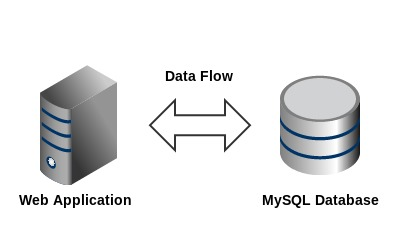
\includegraphics[width=0.8\textwidth]{external-overview.jpg}
    \caption{Connection between application and database}
\end{figure}

To connect to this database using JDBC, you will use the following Java method to pass in important authentication data to authorize access to the data store. At runtime the application requires the username and password pair in \emph{plain-text}. 

\begin{lstlisting}
	Connection conn = DriverManager.getConnection(url, "username", "password");
\end{lstlisting} \\


For our simple case, we have stored the password in \emph{plain-text} in the configuration file. Our application is made of many internal components that are involved with the credential  information we want to protect. The application has following components that are involved with the storage of the credentials:

\begin{itemize}
  \item Web Browser 
  \item Tomcat Servlet
  \item Tomcat Container 
  \item Java Process
  \item Operating System
  \item Hardware
\end{itemize}










\section*{4 Future Plans}





\section*{5 Feedback Required}






%%%%%%%%%%%%%%%%%%%%%%%%%%%%%%%%%%%%%%%%%%%%%%%%%%%%%%%
\backmatter
%%%%%%%%%%%%%%%%%%%%%%%%%%%%%%%%%%%%%%%%%%%%%%%%%%%%%%%

%\bibliographystyle{ieeetr}
\bibliographystyle{acm}
\bibliography{bib}
\end{document}
